\section{Analysis of performance}

To more accurately measure the performance of each language, we introduce benchmarking.

In computer science, benchmarking refers to the evaluation of
the performance of an object by running a computer program or
manipulating some specific behavior\cite{fleming1986not}.
It is done through a series of comparative experiments with
controlled variables usually involving several iterative rounds
in order to draw reproducible and precise conclusions.
In addition, it focuses on a particular procedure and
should exclude the influence of unrelated procedures on
the benchmark test.
This requires that the benchmark test should have a
clear idea of how the underlying workings work and avoid errors
due to the uncertainty of the system's state.

\subsection{Benchmarking Setup}

%\begin{table}[htb]
%    \centering
%    \caption{Benchmarking platform}
%    \label{tab:platform}
%    \begin{tabular}{cc}
%        \hline
%        CPU    & ECS 4 Cores 3.0GHz \\
%        Memory & 16GiB              \\
%        OS     & CentOS 8.2 64bit   \\
%        \hline
%    \end{tabular}
%\end{table}

This test uses Python scripts to perform coarse-grained
batch testing uniformly and uses built-in process tools
to invoke Linux system commands without relying on
third-party libraries, which has high testing efficiency
and is, therefore, suitable for large amounts of data.
Each test program was executed six times, and the results
were averaged to avoid bias.
Each benchmark test was
executed with larger and smaller scale inputs.
We choose the host with a 4-core 3.0GHz CPU, 16GB RAM, CentOS 8.2.
For the compiler environment of the programming
language, see Table\ref{tab:version}.

\begin{table}[htbp]
    \caption{Language versions and dependencies}
    \label{tab:version}
    \begin{center}
        \begin{tabular}{ccc}
            \toprule
            Language   & Version         & Dependency \\
            \midrule
            Python     & CPython3.8      & -          \\
            Java       & OpenJDK17       & -          \\
            C++        & Clang14/GCC11.2 & -          \\
            JavaScript & Node16          & -          \\
            Go         & Go1.17          & -          \\
            Swift      & Swift5.5        & -          \\
            Dart       & Dart2.16        & -          \\
            Rust       & Rust1.54        & MinGW7.3   \\
            Kotlin     & Kotlin1.6       & OpenJDK8   \\
            \bottomrule
        \end{tabular}
    \end{center}
\end{table}

For the same language with different compilers or compilation methods, compare their differences (e.g. C++, Dart). For the remaining languages, we classify them according to the programming language type system. Because for multiple languages with the same type system and compilation method, there should be overlap in their scope of application in practice, the comparative analysis.

The benchmarking metrics for computer languages come from one of the
more popular cross-language benchmarking suites available -
the Computer Language Benchmarking Game\cite{gouy2017computer}.
For each language, there are four metrics.


\begin{enumerate}
    \item Compiler. marked after the programming language, if not marked then the official compiler is used.
    \item Size. The size of the source code after gzip compression. For the same algorithm, the smaller the amount of code used by a programming language, the more syntactically expressive the language is, in general.
    \item CPU. The time required to run the algorithm. Takes the minimum value of multiple runs. Includes startup time.
    \item Memory. The peak space consumption to run the algorithm. Takes the maximum of multiple runs.
\end{enumerate}

\subsection{Memory allocation test}
The idea is derived from Hans-J. Boehm's GC bench algorithm.
The memory allocation capacity and garbage collection capacity are measured by repeatedly allocating and deallocating large amounts of space.
The steps are described in Algorithm 1.
We obtain the CPU and memory overhead results for the selected MPLs
by taking n=21 and n=14, respectively, as shown in Table~\ref{tab:binary-trees-1} and Table~\ref{tab:binary-trees-2}.

\begin{figure}[htbp]
    \centerline{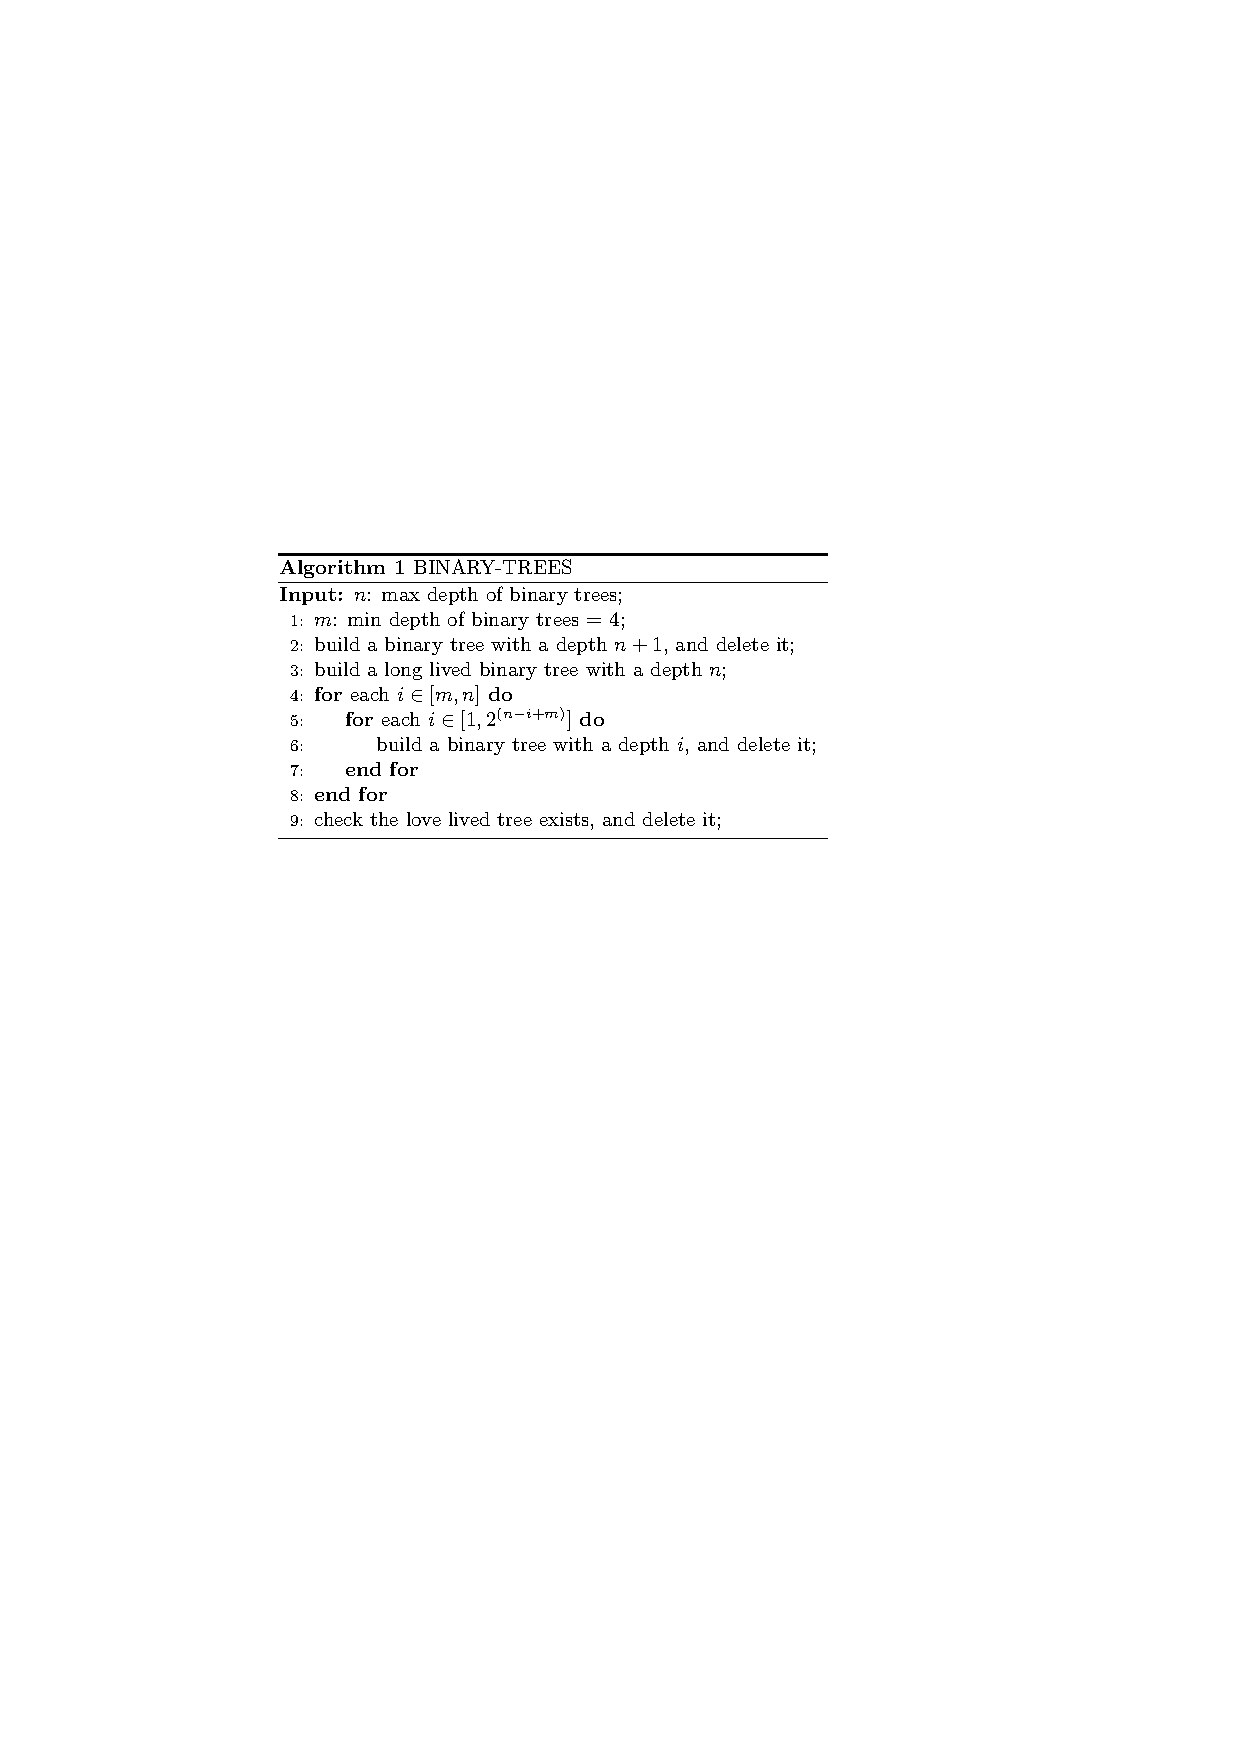
\includegraphics[scale=0.8]{figures/binary-trees}}
    \label{fig:binary-trees}
\end{figure}

\begin{table}[ht]
    \caption{Memory allocation test - large input}
    \label{tab:binary-trees-1}
    \begin{center}
        \begin{tabular}{lrrrr}
            \toprule
            lang      & n  & size(B) & cpu(s)  & mem(KB) \\
            \midrule
            cpp-clang & 21 & 654     & 16.438  & 263580  \\
            cpp-gcc   & 21 & 654     & 22.181  & 263620  \\
            dart-aot  & 21 & 1212    & 45.461  & 799012  \\
            dart-jit  & 21 & 1212    & 61.531  & 1626352 \\
            go        & 21 & 482     & 50.955  & 220548  \\
            java      & 21 & 552     & 5.607   & 2015512 \\
            js-node   & 21 & 711     & 36.391  & 1130788 \\
            kt-jvm    & 21 & 494     & 8.923   & 1783144 \\
            python3   & 21 & 589     & 169.912 & 442180  \\
            rust      & 21 & 751     & 7.796   & 132508  \\
            swift     & 21 & 714     & 63.608  & 733144  \\
            \bottomrule
        \end{tabular}
    \end{center}
\end{table}

\begin{table}[htbp]
    \caption{Memory allocation test - small input}
    \label{tab:binary-trees-2}
    \begin{center}
        \begin{tabular}{lrrrr}
            \toprule
            lang      & n  & size(B) & cpu(s) & mem(KB) \\
            \midrule
            cpp-clang & 14 & 654     & 0.087  & 1200    \\
            cpp-gcc   & 14 & 654     & 0.104  & 3928    \\
            dart-aot  & 14 & 1212    & 0.120  & 1680    \\
            dart-jit  & 14 & 1212    & 0.644  & 170008  \\
            go        & 14 & 482     & 0.214  & 7232    \\
            java      & 14 & 552     & 0.155  & 47968   \\
            js-node   & 14 & 711     & 0.717  & 90512   \\
            kt-jvm    & 14 & 494     & 0.249  & 36040   \\
            python3   & 14 & 589     & 0.911  & 14420   \\
            rust      & 14 & 751     & 0.042  & 1176    \\
            swift     & 14 & 714     & 0.299  & 17616   \\
            \bottomrule
        \end{tabular}
    \end{center}
\end{table}

As we can see from the Table\ref{tab:binary-trees-1} and Table~\ref{tab:binary-trees-2},
Java has the best memory allocation and management
speed among these programming languages.
However, Java's memory consumption is relatively the largest among these languages.
This is due to the unique memory model of the JVM, which divides the heap area into
different generations and uses different garbage collection algorithms for each generation.
The advantage of this is obvious, it can greatly increase the efficiency of garbage
collection. But at the same time, it takes up more memory than is actually needed for the division.
Since Kotlin and Java are both based on the JVM, they have similar performance figures.
Kotlin is based on Java8, while Java is based on Java17. From Java9 onwards, the default JVM GC is G1.
It has better response time than Parallel, but consumes more memory at the same time.
This is in line with the data in the table that Kotlin's time overhead is slightly higher
than Java's and memory overhead is slightly lower.

In Table~\ref{tab:binary-trees-1} and Table~\ref{tab:binary-trees-2},
for the two different compilers for C++, Clang and GCC, the memory overhead is almost the same.
This is because both of them manage memory manually.
However, Clang has a lower time overhead than GCC. This comes from compiler optimizations,
and Clang's optimizations are better than GCC's. In addition, the architecture of the compilers is different:
Clang-LLVM uses a low-coupling front- and back-end architecture, while GCC uses a front- and back-end coupling
architecture.
We can see that compile-time optimization of the compiler takes a more important role for native compiled languages.

Rust, Go and Swift, which are also strongly typed, natively compiled MPLs,
use three different memory management models.
The test results for all three are highly dependent on their
respective memory models.
Go uses a garbage collector.
Although Go is a natively compiled language, there is an additional runtime to support garbage collection.
Compared to Java, Go uses a more conservative garbage collection strategy and does
not aggressively use a space-for-time approach, resulting in decent space consumption
and less optimistic runtimes for memory allocation in Table~\ref{tab:binary-trees-1} and Table~\ref{tab:binary-trees-2}.
Rust uses an ownership mechanism,
unlike C/C++, which is purely manually managed, and unlike Go's garbage collection.
In terms of the underlying implementation, Rust does not actually maintain a runtime
to manage space but rather determines the timing of unallocating memory at compile
time through a complex arithmetic ownership algorithm. As a result, Rust's memory
management is overhead-free. In fact, Rust's compiler backend uses LLVM, the same
backend as the Clang-LLVM tested above, and it is also clear from the test data that
Rust performs almost identically to Cpp-Clang in Table~\ref{tab:n-body-1} and Table~\ref{tab:n-body-2}.
However,due to its ownership mechanism, Rust is better at memory allocation. For Swift,
the memory management mechanism is different from all of the above. Swift allocates
and deallocates memory by maintaining a runtime reference count. In addition,
Swift forces reference counts to be updated atomically instead of Rust's compiler
management of thread safety, which results in high CPU overhead in Table~\ref{tab:binary-trees-1} and Table~\ref{tab:binary-trees-2}. This shows that
Swift has a higher runtime overhead compared to Rust, confirming the data that
Swift performs poorly compared to Rust.

\subsection{Floating-point operation test}

The idea comes from the Symplectic Integration algorithm of K. P. Rauch
and D. P. Hamilton.
This algorithm simulates the evolution of multiple planets and checks the correctness of the program by examining the energy of each evolutionary state. The performance bottleneck is mainly in floating-point operations.
The steps are described in Algorithm 2.
We obtain the CPU and memory overhead results
for the selected MPLs by taking n=5e7 and n=5e6, respectively,
as shown in Table~\ref{tab:n-body-1} and Table~\ref{tab:n-body-2}.

\begin{figure}[htbp]
    \centerline{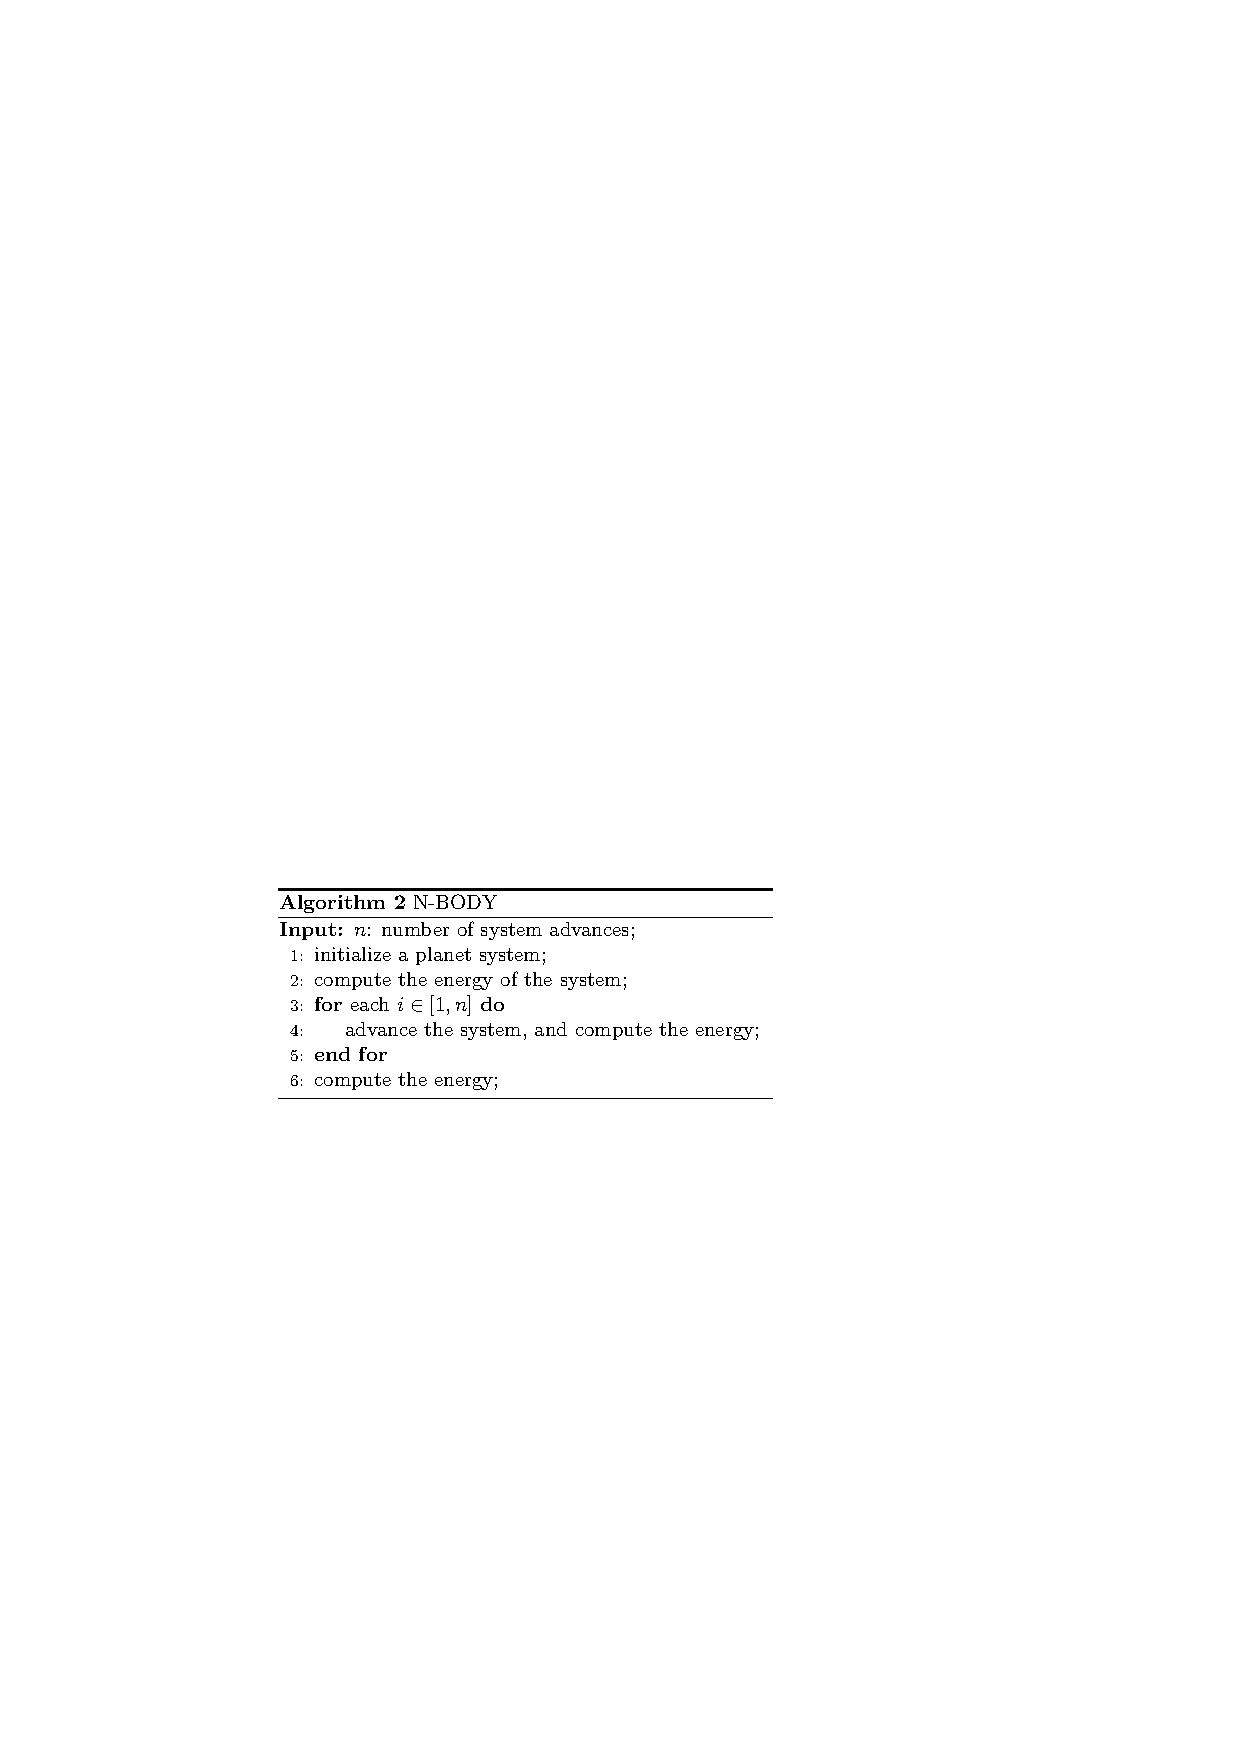
\includegraphics[scale=0.8]{figures/n-body}}
    \label{fig:n-body}
\end{figure}

\begin{table}[ht]
    \caption{Floating-point operation test - large input}
    \label{tab:n-body-1}
    \begin{center}
        \begin{tabular}{lrrrr}
            \toprule
            lang      & n        & size(B) & cpu(s)  & mem(KB) \\
            \midrule
            cpp-clang & 50000000 & 1173    & 5.926   & 1236    \\
            cpp-gcc   & 50000000 & 1173    & 7.555   & 1228    \\
            dart-aot  & 50000000 & 1266    & 10.220  & 9308    \\
            dart-jit  & 50000000 & 1266    & 13.193  & 143436  \\
            go        & 50000000 & 1310    & 6.581   & 1128    \\
            java      & 50000000 & 1430    & 7.816   & 37260   \\
            js-node   & 50000000 & 1268    & 8.550   & 39956   \\
            kt-jvm    & 50000000 & 1124    & 6.914   & 37068   \\
            python3   & 50000000 & 1196    & 541.319 & 7780    \\
            rust      & 50000000 & 1480    & 5.818   & 1024    \\
            swift     & 50000000 & 1192    & 9.585   & 6308    \\
            \bottomrule
        \end{tabular}
    \end{center}
\end{table}


\begin{table}[htbp]
    \caption{Floating-point operation test - small input}
    \label{tab:n-body-2}
    \begin{center}
        \begin{tabular}{lrrrr}
            \toprule
            lang      & n       & size(B) & cpu(s) & mem(KB) \\
            \midrule
            cpp-clang & 5000000 & 1173    & 0.621  & 1204    \\
            cpp-gcc   & 5000000 & 1173    & 0.766  & 1204    \\
            dart-aot  & 5000000 & 1266    & 1.033  & 9216    \\
            dart-jit  & 5000000 & 1266    & 1.918  & 143256  \\
            go        & 5000000 & 1310    & 0.661  & 816     \\
            java      & 5000000 & 1430    & 0.880  & 37460   \\
            js-node   & 5000000 & 1268    & 0.941  & 39864   \\
            kt-jvm    & 5000000 & 1124    & 0.826  & 37064   \\
            python3   & 5000000 & 1196    & 52.530 & 7800    \\
            rust      & 5000000 & 1480    & 0.579  & 1020    \\
            swift     & 5000000 & 1192    & 0.976  & 6308    \\
            \bottomrule
        \end{tabular}
    \end{center}
\end{table}

In Table~\ref{tab:binary-trees-1} and Table~\ref{tab:binary-trees-2},
Java's time overhead is not very high and does not fall too far behind natively compiled languages. The performance bottleneck of algorithmic programs with short execution time is mainly the JVM startup time and the JIT-optimized warm-up time, and for algorithms that have already done so, Java's execution speed does not lag behind that of natively compiled languages. Java runs in two steps. In the first step, the source code is compiled into bytecode, and in the second step, the JVM interprets and executes the bytecode. In the process of interpreting and executing the bytecode, JVM will receive the runtime information of the collected code, and if it finds that some bytecode is executed more frequently, it will choose to compile this part of the bytecode and compile it into native code, which will be called directly when it is executed again. The so-called performance optimization of Java is mainly in the bytecode, while the source to bytecode stage is only a simple optimization.

In Table~\ref{tab:binary-trees-1} and Table~\ref{tab:binary-trees-2},
there is a significant performance gap between JavaScript and Python. JavaScript runs on Google's V8 engine, which executes JavaScript code much like the JVM executes bytecode, using the same JIT optimization technique. So compared to Python, which does not use JIT optimization, it has a huge performance improvement, even with Java and natively compiled languages with similar floating point performance. In fact, the speed of scripting languages is not a performance bottleneck in most application scenarios. However, in recent years, JavaScript has become the "assembly of the web", and more and more languages are being compiled into JavaScript, such as Kotlin and Dart, so more and more business logic needs to be executed in JavaScript. This makes JavaScript burdened with tedious business-related logic, and optimization of JavaScript is the trend.

\subsection{Comprehensive test}

The Mandelbrot Set is drawn on a resolution N×N bitmap. the coordinates of the image on the complex axis are [-1.5-i,0.5+i]. For each pixel, a certain number of iterations are performed to determine the gray level of the current pixel. The output in PBF format is performed byte by byte. The correctness is checked by comparing it with the standard output. The performance bottleneck of this test is in floating point operations, memory allocation, and IO.
The steps are described in Algorithm 3.
We obtain the CPU and memory overhead results
for the selected MPLs by taking n=16000 and n=4000, respectively,
as shown in Table~\ref{tab:mandelbrot-1} and Table~\ref{tab:mandelbrot-2}.

\begin{figure}[htbp]
    \centerline{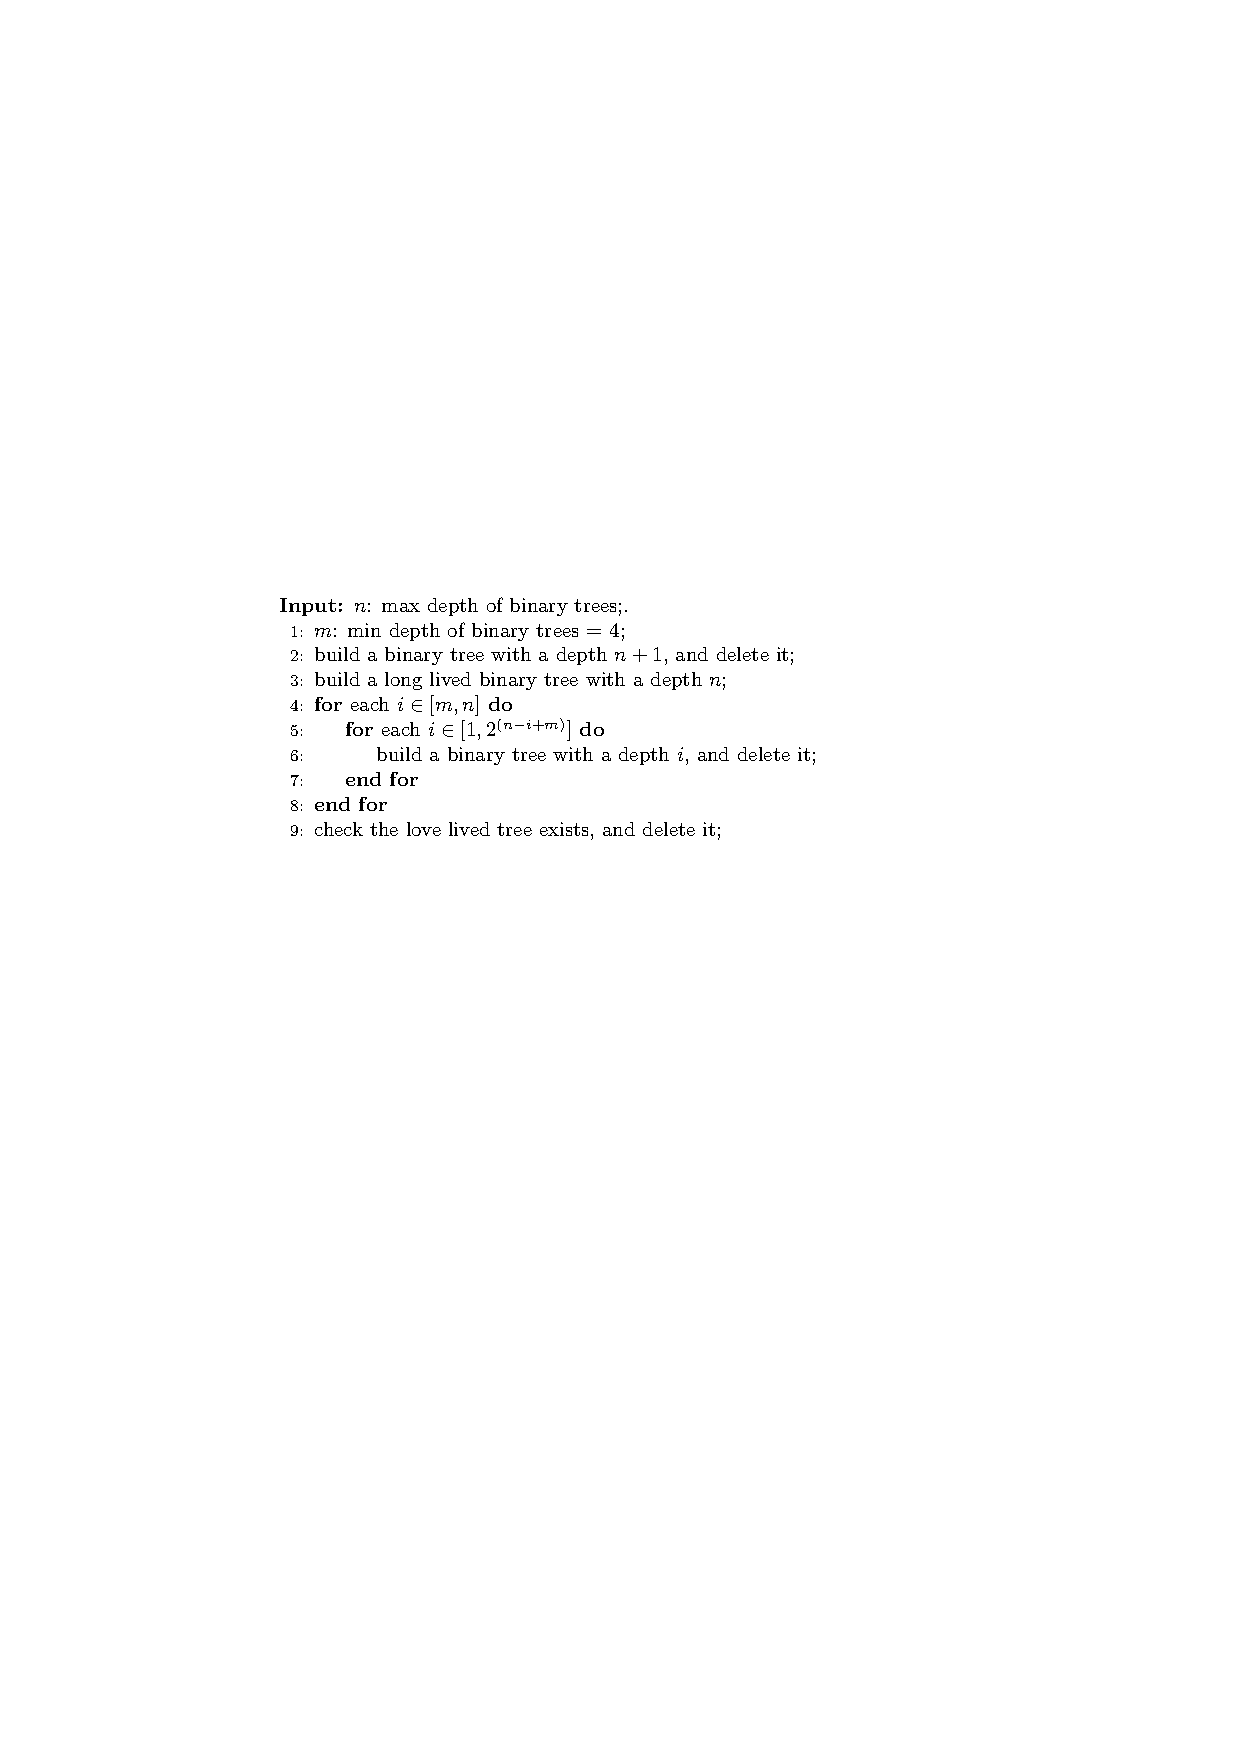
\includegraphics[scale=0.8]{figures/mandelbrot}}
    \label{fig:mandelbrot}
\end{figure}

\begin{table}[ht]
    \caption{Comprehensive test - large input}
    \label{tab:mandelbrot-1}
    \begin{center}
        \begin{tabular}{lrrrr}
            \toprule
            lang      & n     & size(B) & cpu(s)  & mem(KB) \\
            \midrule
            cpp-clang & 16000 & 822     & 13.900  & 30172   \\
            cpp-gcc   & 16000 & 822     & 13.931  & 28696   \\
            dart-aot  & 16000 & 454     & 154.089 & 17240   \\
            dart-jit  & 16000 & 454     & 151.501 & 148144  \\
            go        & 16000 & 823     & 19.598  & 32412   \\
            java      & 16000 & 665     & 27.834  & 34264   \\
            js-node   & 16000 & 373     & 130.638 & 42020   \\
            kt-jvm    & 16000 & 407     & 30.032  & 28432   \\
            python3   & 16000 & 688     & 702.599 & 47780   \\
            rust      & 16000 & 868     & 11.904  & 38528   \\
            swift     & 16000 & 394     & 26.277  & 6200    \\
            \bottomrule
        \end{tabular}
    \end{center}
\end{table}


\begin{table}[htbp]
    \caption{Comprehensive test - small input}
    \label{tab:mandelbrot-2}
    \begin{center}
        \begin{tabular}{lrrrr}
            \toprule
            lang      & n    & size(B) & cpu(s) & mem(KB) \\
            \midrule
            cpp-clang & 4000 & 822     & 0.880  & 1552    \\
            cpp-gcc   & 4000 & 822     & 0.881  & 1192    \\
            dart-aot  & 4000 & 454     & 10.276 & 17380   \\
            dart-jit  & 4000 & 454     & 10.096 & 148084  \\
            go        & 4000 & 823     & 1.260  & 2420    \\
            java      & 4000 & 665     & 1.827  & 34352   \\
            js-node   & 4000 & 373     & 8.763  & 42540   \\
            kt-jvm    & 4000 & 407     & 2.419  & 28448   \\
            python3   & 4000 & 688     & 46.273 & 12172   \\
            rust      & 4000 & 868     & 0.757  & 4388    \\
            swift     & 4000 & 394     & 1.661  & 6240    \\
            \bottomrule
        \end{tabular}
    \end{center}
\end{table}

For the same Dart code, it is compiled in two different ways,
using JIT and AOT. As for the time and memory overhead in Table~\ref{tab:mandelbrot-1} and Table~\ref{tab:mandelbrot-2},
both have similar performance. This is caused by the compilation mechanism of Dart. In fact, the running mechanism of Dart is different from the traditional way. The traditional AOT is to compile the source code directly into the object code on the target machine, which can be called and run independently by the operating system directly. However, for Dart, whether it is AOT or JIT, only the compilation time is different, and it will eventually run on the virtual machine. In fact, when the compilation time is negligible, the time overhead of AOT and JIT is approximately equal. But this way of running has its unique disadvantage. It will significantly increase the running overhead of AOT mode, but this makes AOT compilation has strong runtime support. Because of this feature, the Dart VM can save the current runtime state, and the next time the VM is started, it can directly load the last state without restarting. This is mainly for a better development experience. The incremental compilation feature allows the runtime results to change almost in real time as the code is changed. Dart is a language for the front-end cross-platform framework Flutter. With such a mechanism, code changes can feed back to the UI in real-time, which is hard to do with other languages.

In industrial applications, the performance bottleneck in most scenarios is compile-related, including not only compile-time but also run-time. The impact of compilation on programming language efficiency is again multifaceted. First, the same programming language with different compilers will often have different object code and thus different runtime efficiency. This is often due to different compile-time optimizations; for example, for C++, there is a significant performance difference in the object code obtained by compiling with Clang-LLVM as opposed to compiling with GCC. Second, the same programming language can run not only in AOT, but also in JIT. For example, for Kotlin, it can be compiled not only as bytecode to run on JVM, but also programmed as JavaScript code to run on the browser, or even Kotlin Native, which can run as native code. In this way, the different compilation methods have a greater impact on efficiency.

The impact of memory management on programming language performance is huge. First, there is the matter of memory allocation on the heap. For languages with VM, memory allocation is an advantage compared to non-VM languages. This is because VM languages provide memory pools that host the memory allocation, whereas non-VM languages do not have such an advantage. Of course, for scenarios where memory on the heap is used frequently, non-VM languages tend to use custom or third-party provided memory pooling frameworks, and the performance gap in the industry is not as pronounced. But managed memory is not always an advantage. When a memory thrash occurs, the VM will frequently GC, which also affects performance. And, memory pools tend to have a larger memory overhead. Second, there is the principle of locality about memory. CPU will put all the adjacent data into cache, and if the memory is accessed sequentially, it greatly improves the hit rate of cache, thus improving the performance.
